\chapter{Zestawienie zbiorcze i podsumowanie}

\section{Oferowane funkcjonalności}

Omówione w ramach niniejszej pracy biblioteki różnią się typem i liczbą oferowanych funkcjonalności. Tabela \ref{fun:sum} zbiorczo podsumowuje poszczególne omówione w poprzednich rozdziałach aspekty.

\begin{longtable}{c | c | c | c}
	\centering
	\multirow{2}{*}{\makecell{Funkcjonalność}} & \multicolumn{3}{c}{Biblioteka} \\
	\cline{2-4}
	 &  Shogun & Shark-ML & Dlib \\
	\hline
	\makecell{Odczyt \\ danych} & \makecell{std::vector, \\ wsparcie dla \\ formatu CSV} & \makecell{surowe \\ tablice, \\ wsparcie dla \\ formatu CSV, \\ wsparcie \\ dla HTTP} & \makecell{std::vector, \\ wsparcie dla \\ formatu CSV} \\
	\hline
	{Normalizacja} & min-max & \makecell{przedział \\ jednostkowy, \\ jednostkowa \\ wariancja, \\ zerowa \\ średnia i \\ wybrana \\ wariancja} & standaryzacja \\
	\hline
	\makecell{Redukcja \\ wymiarowości} & \makecell{PCA, Kernel PCA, \\ MDS, IsoMap, \\ ICA, Factor analysis, \\t-SNE} & \makecell{PCA, Liniowa \\ analiza \\ dyskryminacyjna} & \makecell{PCA, Liniowa \\ analiza \\ dyskryminacyjna, \\ Mapowanie \\ Sammona} \\
	\hline
	\makecell{Regularyzacja} & \makecell{L1 i L2 \\ automatyczna} & \makecell{L1 i L2} & L2 \\
	\hline
	\makecell{Regresja \\ liniowa} & Tak & Tak & Tak \\
	\hline
	\makecell{Regresja \\ logistyczna} & Tak & Tak & Nie \\
	\hline
	\makecell{Maszyna \\ wektorów \\ nośnych} & Tak & Tak & Tak \\
	\hline
	\makecell{Algorytm \\ K-najbliższych \\ sąsiadów} & Tak & Tak & Nie \\
	\hline
	\makecell{Algorytm \\ zbiorowy} & \makecell{Wzmacnianie \\ gradientu, \\ losowy las} & \makecell{Losowy \\ las} & Nie \\
	\hline
	\makecell{Sieć \\ neuronowa} & Tak & Tak & Tak \\
	\hline
	\makecell{Jądrowa \\ regresja \\ grzbietowa} & Nie & Nie & Tak \\
	\hline
	\makecell{Błąd \\ średniokwadratowy} & Tak & Tak & Nie \\
	\hline
	\makecell{Średni \\ błąd \\ bezwzględny} & Tak & Tak & Nie \\
	\hline
	\makecell{Błąd typu \\ zero-jeden} & Nie & Tak & Nie \\
	\hline
	\makecell{Błąd \\ dyskretny} & Nie & Tak & Nie \\
	\hline
	\makecell{Entropia \\ krzyżowa} & Nie & Tak & Nie \\
	\hline
	\makecell{Kawałkami \\ liniowa \\ funkcja straty} & Nie & Tak & Nie \\
	\hline
	\makecell{Średnio-\\kwadratowy \\ błąd typu \\ kawałkami \\ liniowej \\ funkcji straty} & Nie & Tak & Nie\\
	\hline
	\makecell{Kawałkami \\ liniowa \\ funkcja straty \\ typu epsilon} & Nie & Tak & Nie\\
	\hline
	\makecell{Średnio-\\kwadratowy \\ błąd kawałkami \\ liniowej funkcji \\ straty typu \\ epsilon} & Nie & Tak & Nie\\
	\hline
	\makecell{Funkcja \\ straty \\ Hubera} & Nie & Tak & Nie\\
	\hline
	\makecell{Funkcja \\ straty \\ Tukeya} & Nie & Tak & Nie\\
	\hline
	\makecell{Logarytmiczna \\ funkcja \\ straty} & Tak & Nie & Nie\\
	\hline
	\makecell{Metryka $R^2$} & Tak & Tak & Nie\\
	\hline
	\makecell{Dokładność} & Tak & Nie & Tak \\
	\hline
	\makecell{Pole pod \\ wykresem \\ ROC} & Tak & Tak & Tak* \\
	\hline
	\makecell{Sprawdzian \\ krzyżowy \\ k-krotny} & Tak & Tak & Tak \\
	\caption{Zbiorcze porównanie funkcjonalności bibliotek}
	\label{fun:sum}
\end{longtable} 

* - konieczność przeliczenia pola na podstawie uzyskanych punktów pomiarowych wykresu funkcji.

Analizując dane zebrane w tabeli \ref{fun:sum} można zauważyć, że biblioteki Shogun oraz Shark-ML są bardzo zbliżone do siebie typem i liczbą dostępnych metod uczenia maszynowego, jednak Shark-ML posiada więcej rodzajów błędów możliwych do wykorzystania jako funkcje strat, pozwalając na większą swobodę względem dostosowywania procesu uczenia. Najmniejszą liczbą funkcjonalności charakteryzuje się biblioteka Dlib, posiadająca jedynie podzbiór algorytmów dostępnych w innych projektach. Ponadto, posiada ona bardzo ubogie możliwości analizy sprawności modeli, wymagając od użytkownika napisania własnych procedur przetwarzania uzyskanych danych, jak np. procedura obliczania pola pod wykresem krzywej charakterystycznej odbiornika.

\section{Porównanie wyników dla zadanych przykładów}

W celu przetestowania sprawności poszczególnych bibliotek, użyto ich do stworzenia i ewaluacji modeli regresji liniowej oraz maszyny wektorów nośnych dla zestawów danych opisanych w rozdziale 3. Dla każdego modelu użyto 80\% zestawu danych w celu treningu, oraz pozostałe 20\% jako dane testowe. Tabela \ref{tab:models} przedstawia zbiorcze zestawienie uzyskanych wyników ewaluacji. Wyjście programów zostało zaprezentowane na rysunkach \ref{fig:shogun_linear_svm}, \ref{fig:shark_linear_svm} oraz \ref{fig:dlib_linear_svm}.

\begin{longtable}{c | c | c }
	\centering
	\multirow{2}{*}{\makecell{Biblioteka}} & \multicolumn{2}{c}{Metoda uczenia maszynowego} \\
	\cline{2-3}
	& Regresja liniowa & Maszyna wektorów nośnych \\
	\hline
	\makecell{Shogun} & \makecell{Dane treningowe: \\ MSE = 0,903031; $R^2$ = 0,407058 \\ Dane testowe: \\ MSE = 1,26897; $R^2$ = -0.127851} & \makecell{Dane treningowe: \\ AUC ROC: 1 \\ Dane testowe: \\ AUC ROC: 0,5} \\
	\hline
	\makecell{Shark} & \makecell{Dane treningowe: \\ MSE = 0,38728; $R^2$ = 0,745707 \\ Dane testowe: \\ MSE = 0,449118; $R^2$ = 0,60082} & \makecell{Dane treningowe: \\ AUC ROC: 1 \\ Dane testowe: \\ AUC ROC: 0,5} \\
	\hline
	\makecell{Dlib} & & 
	\label{tab:models}
\end{longtable} 

\begin{figure}[!ht]
	\centering
	\begin{minipage}{0.32\textwidth}
		\centering
		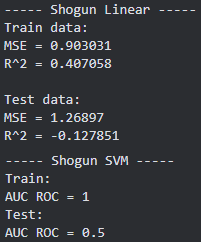
\includegraphics[width=\linewidth]{Rozdzial7/shogun}
		\caption{Wynik działania programu dla biblioteki Shogun}
		\label{fig:shogun_linear_svm}		
	\end{minipage}%
    \hspace{0.02\textwidth}
	\begin{minipage}{0.32\textwidth}
		\centering
		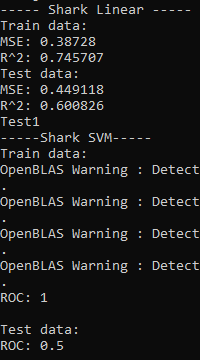
\includegraphics[width=0.7\linewidth]{Rozdzial7/shark}
		\caption{Wynik działania programu dla biblioteki Shark}
		\label{fig:shark_linear_svm}		
	\end{minipage}
\end{figure}

DOPISAĆ DALEJ !!!!!

\begin{figure}[!ht]
	
\end{figure}


\section{Wymagany nakład pracy i jakość źródeł}

W procesie pracy z poszczególnymi bibliotekami zauważono, że najmniejszą ilością potrzebnego wkładu pracy charakteryzowała się biblioteka Shark-ML. Wynika to z bardzo przyjaznej dla użytkownika składni, oraz dokładnej dokumentacji dostępnej na stronie internetowej projektu, wraz z przykładami wykorzystania poszczególnych metod. Biblioteka także bez jakichkolwiek problemów została zbudowana i zainstalowana na systemie operacyjnym Ubuntu 22.04 w środowisku WSL, pozwalając bardzo szybko przejść do docelowej pracy.

Drugą biblioteką pod względem koniecznego wkładu czasu okazał się zestaw narzędziowy Dlib. Posiada on stronę projektu z wylistowanymi klasami oraz funkcjami dostępnymi w bibliotece, jednak opis działania poszczególnych metod jest bardzo pobieżny, oraz brakuje dostępnych przykładów. Składnia biblioteki może stanowić wyzwanie dla użytkownika, gdyż nie zawsze jest oczywista, i momentami utrudnia analizę realizowanych przez program operacji.

Jako najbardziej wymagającą bibliotekę uznano Shogun. W chwili pisania niniejszej pracy, zarówno oficjalne repozytorium projektu jak i repozytorium dystrybucji dla systemu operacyjnego Ubuntu okazało się być niekompletne. Uniemożliwiło to zainstalowanie biblioteki za pomocą wbudowanego managera pakietów oraz zbudowanie jej ze względu na nienaprawione zależności do przeniesionych repozytoriów stron trzecich. Mimo przyjaźniejszej składni niż w przypadku Dlib, wspomniany wcześniej mankament sprawia, że w celu pobrania biblioteki konieczne okazało się zainstalowanie specjalnego managera pakietów \textit{nix} posiadającego starszą wersję projektu Shogun dostępną na swoim repozytorium. Z racji braku dostępnej online dokumentacji projektu Shogun oraz faktu, że generowane przykłady nie odnoszą się do API biblioteki lecz używają jej w kompletnie odrębny, nienaturalny dla projektu sposób, ustalenie funkcjonalności oraz sposobu realizacji poszczególnych zadań uczenia maszynowego musiało zostać oparte praktycznie wyłącznie o materiały dostępne w formie książkowej. Znacznie utrudnia i wydłuża to proces zastosowania biblioteki do jakiegokolwiek projektu.